\documentclass{article}
\title{64-bit Counter v1.0}
\author{Peter Todd}
\date{}
\usepackage{graphicx}
\usepackage{url}
\begin{document}
   \maketitle

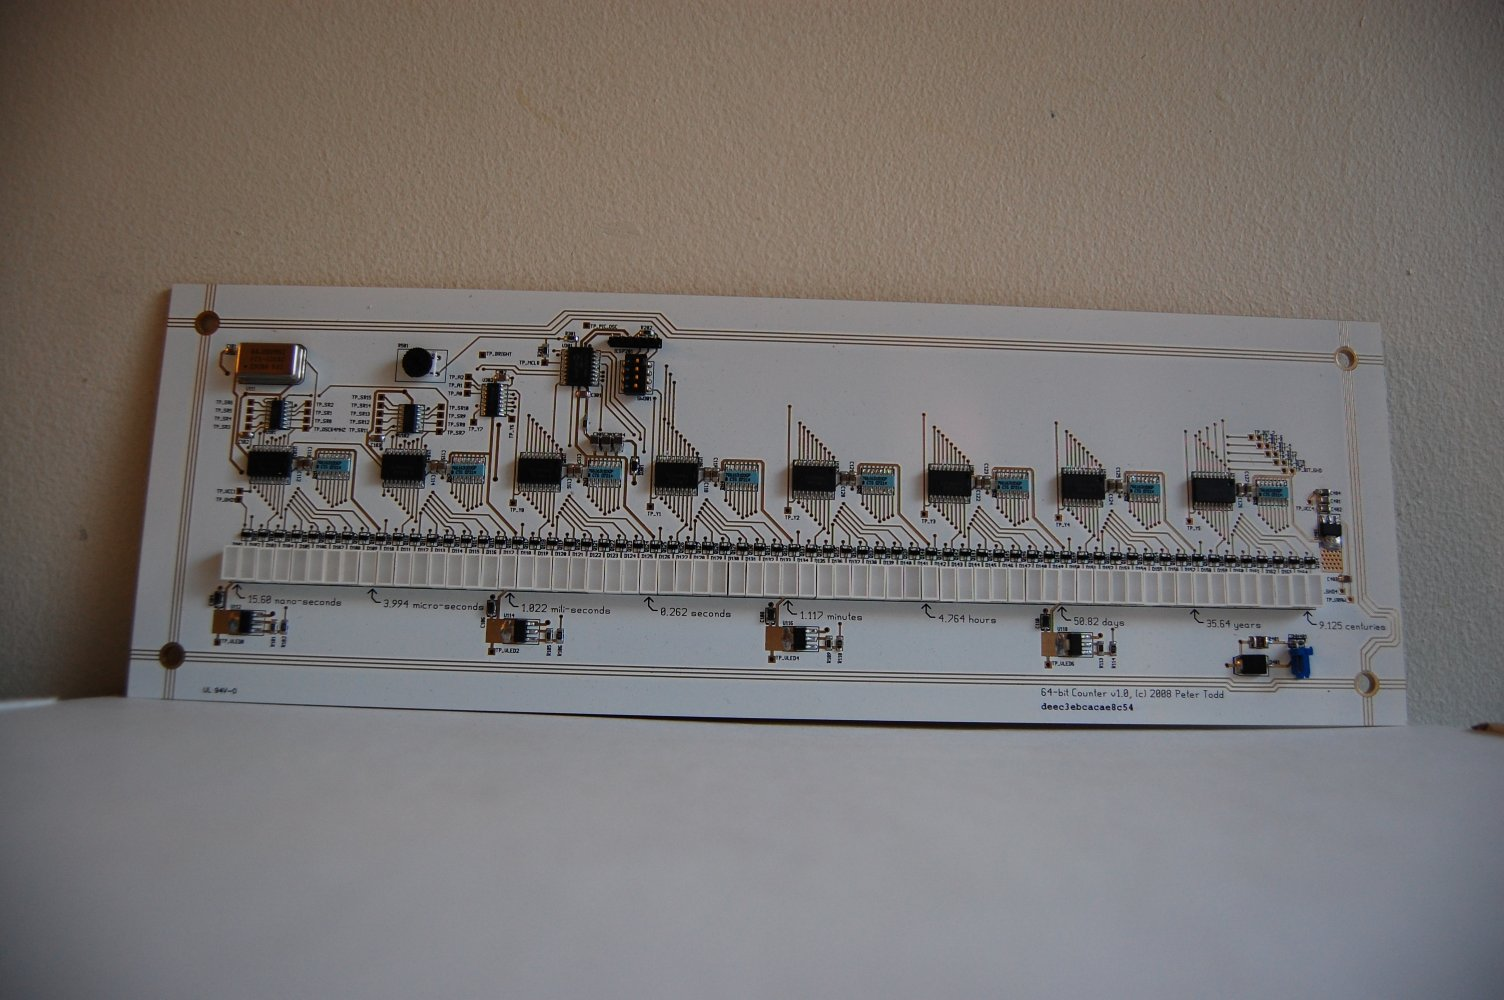
\includegraphics[width=4.25in]{figures/front.eps}

\section{Overview}

The 64-bit Counter takes a 64mhz clock, and divides that clock in a binary
sequence, displaying each division level on an LED. The count reached is
permenantly stored in an EEPROM, maintaining state.

\subsection{Specifications}

\begin{itemize}
	\item Dimensions: 15"x5"
	\item Power source: 6VDC 2A wall adapter
\end{itemize}

\section{Mounting}

Use the holes provided. Power is supplied via the blue plug on the lower right
hand corner.

\section{Maintenance}

The 64-bit Counter requires no maintenance. If cleaning is required water will
not harm the electronics so long as the device is off and allowed to dry
throughly before applying power again. It's best to simply use a damp cloth.

\pagebreak

\end{document}
